\documentclass[journal]{IEEEtran}
\usepackage[T1]{fontenc}
\usepackage[utf8]{inputenc}
\usepackage{cite,booktabs,array,graphicx}
\usepackage{tikz}
\usetikzlibrary{arrows.meta,positioning,fit}
\usepackage[hidelinks]{hyperref}
\hypersetup{pdftitle={Organizational Complexity, Data Growth, and Decision Support Systems},pdfauthor={}}
\title{Organizational Complexity, Data Growth, and Decision Support Systems: A Critical Integrative Review of Their Feedback Dynamics}
\author{Unattributed review manuscript}
\begin{document}
\maketitle
\begin{abstract}
Decision support systems (DSS) are commonly described through successive technologies, but technological chronology alone does not explain their changing organizational role. This critical integrative review examines how organizational complexity, data growth, and decision support can form reinforcing and balancing feedback relationships. A purposive, full-text corpus of 24 works integrates organizational information-processing theory, primary DSS frameworks, architecture studies, organizational cases, and formal or simulated endogenous-data mechanisms. The synthesis distinguishes organizational interdependence and equivocality from record volume, and technical throughput from usable organizational processing capacity. Five overlapping information-processing configurations illustrate historical responses: interactive models, codified and collaborative expertise, enterprise analytical integration, data-dependent prediction, and evidence-linked workflow support. Across them, additional data and computational capacity can alleviate a constraint while transferring work to interpretation, integration, maintenance, or coordination. The reverse relationship is conditional: decision policies can shape future observations, and coupled analytical systems can create new coordination obligations, but neither mechanism proves inevitable growth in organizational complexity or data volume. A link-specific mechanism map, three analytical illustrations including organizational case evidence, and five propositions identify when amplification, stabilization, or simplification is plausible. The contribution is an evidence-traceable synthesis of these relationships, rather than a claim that feedback is newly discovered or that the complete historical loop has been causally established.
\end{abstract}
\begin{IEEEkeywords}
Decision support systems, organizational complexity, information processing, data growth, feedback, sociotechnical systems, endogenous data.
\end{IEEEkeywords}

\section{Introduction}
\IEEEPARstart{O}{rganizations} divide work among people, functions, locations, and increasingly interconnected digital services. Differentiation can create useful specialization while making decisions depend on information held elsewhere. Transactions, monitoring, and coordination generate records that may help manage those dependencies. Yet collecting more records does not automatically create shared understanding, and supporting more decisions can itself introduce interfaces, exceptions, and maintenance obligations. The evolution of DSS therefore raises a reciprocal question: how do organizational information requirements and data-intensive support arrangements change one another?

Foundational organizational information-processing accounts relate task uncertainty and interdependence to the work required to coordinate action \cite{GALBRAITH1974,TUSHMAN1978}. DSS scholarship, meanwhile, documents changing combinations of models, databases, knowledge, interfaces, and collaboration \cite{shim2002,power2004}. Read together, these traditions suggest that architectures evolve partly in response to a mismatch between required and usable processing capacity. However, a mismatch can be addressed by reducing information requirements as well as by increasing technical capacity. The same organizational problem may therefore motivate a more integrated DSS, a simpler decision model, a changed coordination structure, or no technological investment.

The reverse direction matters too. Analytical interventions can change which events are observed and how subsequent decisions are made. Production learning systems also couple data, models, and teams in ways that ordinary software modularity may not contain \cite{perdomo2020,amershi2019}. These mechanisms make feedback plausible, but they do not establish a universal sequence in which complexity always produces more data, which always produces a newer DSS and still more complexity. They operate at different levels, with different evidence and boundary conditions.

This review addresses three questions. RQ1: Under what conditions do organizational complexity and data growth increase decision-support requirements? RQ2: How have DSS information-processing arrangements absorbed, redistributed, or reduced those requirements? RQ3: When can decision support alter future observations and coordination demands, reinforcing or balancing the original pressure? The focus is the organization--data--decision relationship, rather than a ranking of algorithms or an exhaustive inventory of DSS applications.

The contribution has three parts: a construct-consistent comparison across historical DSS arrangements; a mechanism map distinguishing supported directional links from cross-study conjectures; and propositions connecting those links to observable organizational conditions. It does not claim that feedback, sociotechnical reciprocity, or information-processing fit is new. Rather, it connects historical DSS arguments with evidence on endogenous observations and lifecycle coordination, while making countermechanisms explicit.

\section{Review Design and Positioning}
\subsection{Approach and Eligibility}
The study is a critical integrative review using theory-guided, purposive selection. Discovery and assessment for this revision were conducted on 21 October 2026, with publication eligibility ending on that date. The initial DSS catalog contained 67 records; it served as a discovery resource, not as a fully screened or representative study population. Additional targeted searches used Crossref bibliographic metadata, exact-title searches, and authoritative publisher, author, institutional, and archival copies. Searches targeted organizational information processing, DSS history, data-dependent feedback, and organizational implementation. Some metadata queries were rate-limited; unsuccessful access attempts were retained in the search record rather than silently treated as completed searches.

Sources were eligible for substantive synthesis if accessible full text supported at least one of five roles: defining information-processing requirements; explaining a DSS information-processing arrangement; reporting organizational implementation; analyzing feedback in data-dependent decisions; or providing directly comparable prior synthesis. Sources with only metadata or abstracts were recorded as leads, not used as assessed substantive evidence. English-language sources were used; seminal works were retained irrespective of age. The selection was not designed to estimate a publication population, and no exhaustive database search, PRISMA compliance, or independent human dual screening is claimed.

After source-identity reconciliation, the included corpus comprises 24 distinct works: four organizational-theory sources, eight historical/classification sources, five feedback or production-learning sources, two clinical implementation/synthesis sources, three technical mechanism sources, and two additional closely related reviews. Two historical sources also serve in prior-review positioning; they are counted once. These are selection roles, not mutually exclusive research-design categories. An explicit selection register and excluded-candidate record accompany the manuscript. Complete texts were available, but assessment concentrated on the argument, methods, relevant findings, and limitations rather than claiming sentence-by-sentence verification of every document.

\subsection{Extraction and Critical Appraisal}
Extraction recorded the construct or decision problem, information/data relationship, proposed processing response, additional dependencies, countermechanisms, source design, and transfer limits. Supporting locations use published pages where reliable and scan-PDF pages for the assessed MIT working papers. Three foundational theory scans required optical character recognition; evidence was interpreted in context, and exact quotations are avoided. Little's 1969 and Gorry and Scott Morton's 1971 working-paper versions are cited as the versions actually assessed, without substituting journal pagination \cite{little1969,gorry1971}.

Evidence was separated into conceptual theory, historical or secondary synthesis, technical architecture, organizational case evidence, mathematical analysis, and simulation. A theory can justify a relationship without estimating its magnitude; a simulation can expose feedback without demonstrating its organizational prevalence. A publication-content analysis measures research activity, not adoption. This distinction responds to the theory/practice problem identified within DSS scholarship \cite{arnott2008}. No numerical quality score or pooled effect size was constructed across these incompatible designs.

Each mechanism was considered against a rival explanation or boundary: differences in the information required, receiver attention, selection effects, organizational choice, stable feedback, and implementation failure. Source and claim matrices document these checks. Search logs, metadata/provenance, access decisions, and extraction records accompany the paper; they support inspection of the purposive synthesis, not replication of an exhaustive search. Research and drafting were assisted by language-model tools; there was no independent human validation of the screening or coding.

\subsection{Relationship to Existing Reviews}
DSS evolution already has substantial historical and architectural coverage. Shim \emph{et al.} connect organizational and technical developments, including wider collaboration and increasing analytical demands \cite{shim2002}. Power's classification separates the dominant support technology from users, purpose, and deployment \cite{power2004}. Recent reviews discuss architectural autonomy, organizational context, governance, and feedback \cite{Budianto2026,Eze2026}. Accordingly, neither adding an organizational perspective nor drawing a feedback arrow establishes novelty. Table~\ref{tab:prior} identifies the narrower extension attempted here.

The closest reviews are useful for positioning but are not treated as primary confirmation of causal effects. Budianto \emph{et al.}'s strategic-AI framework remains conceptual, and the visible article does not expose enough record-level material to independently reconstruct its reported included-study population \cite{Budianto2026}. Eze \emph{et al.} explicitly adopt an integrative approach, yet the article retains broad cross-category performance numbers alongside a warning against heterogeneous comparison \cite{Eze2026}. Those numbers are not used here. These are appraisal limits of the available documents, not judgments about author intent.

\begin{table*}[t]
\caption{Positioning against assessed prior DSS syntheses}
\label{tab:prior}
\centering\footnotesize\setlength{\tabcolsep}{4pt}
\begin{tabular}{p{.15\textwidth}p{.24\textwidth}p{.26\textwidth}p{.27\textwidth}}
\toprule
Prior synthesis & Organizing lens & Relationships already addressed & Extension attempted in this review \\
\midrule
Shim \emph{et al.} \cite{shim2002} & DSS history, tools, deployment and collaboration & Organizational/technical drivers; more users and data; technology enabling virtual organizations & Link historical mechanisms to explicit information-processing constructs and distinguish forecasts from observations \\
Arnott and Pervan \cite{arnott2008} & Content analysis and discipline quality & Theory/practice gaps; overlapping DSS research categories & Separate research activity from adoption and trace claims to appropriate evidence types \\
Budianto \emph{et al.} \cite{Budianto2026} & Architectural autonomy and strategic business value & Architectural phases, hidden feedback, technical debt and governance & Examine conditional amplification, balancing mechanisms and causal-evidence limits \\
Eze \emph{et al.} \cite{Eze2026} & Taxonomy, architectures, applications and governance & Information-processing theory, hybrid DSS and workflow iteration & Distinguish within-workflow feedback from organization-level coevolution and volume from coordination demands \\
\bottomrule
\end{tabular}
\end{table*}

\section{Constructs and Theoretical Foundations}
\subsection{Organizational Complexity Is Not Data Volume}
Organizational complexity is used here as a multidimensional description: differentiated tasks or units, interdependence among their actions, variation in work, and uncertainty or contested interpretation during coordination. These dimensions can change separately. More employees or transactions may increase scale without increasing reciprocal task interdependence. Conversely, a small multidisciplinary decision can involve substantial ambiguity and conflicting objectives. The review therefore does not assume a single measured complexity index.

Galbraith links uncertainty during task execution to information-processing requirements, including replanning and exception handling \cite{GALBRAITH1974}. Tushman and Nadler relate uncertainty to task characteristics, environment, and interunit interdependence, while distinguishing relevant information from unprocessed data \cite{TUSHMAN1978}. These theories explain why the location and interpretation of knowledge matter, rather than equating an organization with a container of records. Their causal propositions are theory informed by examples and prior research, not direct measurements of the history of DSS.

Daft and Lengel add a crucial distinction: uncertainty involves missing answers to sufficiently specified questions, whereas equivocality involves competing interpretations of the situation or question itself \cite{DAFT1986}. Collecting additional relevant observations may reduce the former. It need not resolve the latter, which can require shared language, negotiation, and changes in problem framing. Treating both as a shortage of bytes invites a technically efficient response to the wrong organizational problem.

\subsection{Data Growth and Usable Processing Capacity}
Data volume denotes the quantity of recorded transactions, observations, or documents available over time. Variety, arrival rate, quality, access restrictions, and provenance are separate properties. A larger archive can contain more duplicates or policy-shaped observations, without a proportionate gain in policy-independent or decision-relevant evidence. The amount stored also differs from the amount presented to a decision maker. A well-designed DSS can expand its underlying archive while reducing the information a person must inspect.

Usable processing capacity denotes the combined ability to acquire, validate, interpret, coordinate, and act on relevant evidence at the required time. It includes computational throughput, memory, storage and networks, but also attention, semantic agreement, expertise, decision authority and maintenance resources. This is an organizing construct, not a measured scalar added across incompatible units. Simon's attention argument explains why increasing communication output can overload downstream receivers rather than improve organizational performance \cite{SIMON1971}.

The distinction also prevents an overly simple hardware-versus-architecture dichotomy. Faster computation can make more frequent replanning feasible; representation and interfaces determine which information can be used; organizational design determines who must interpret and act on it. Galbraith explicitly connects replanning frequency with computer time and input/output work while also warning about receiver overload \cite{GALBRAITH1974}. A technical capacity gain is consequently an affordance whose value depends on the rest of the processing arrangement.

\subsection{Fit, Selection, and Organizational Choice}
A capacity mismatch does not force technological escalation. Galbraith identifies slack resources and self-contained tasks as ways to reduce processing requirements, alongside vertical information systems and lateral relations that increase capacity \cite{GALBRAITH1974}. Tushman and Nadler likewise reject a unique mapping from information requirements to one organizational structure \cite{TUSHMAN1978}. Organizations may accept buffers, narrow a service, change decision rights, coordinate laterally, invest in a DSS, or tolerate poorer performance.

Early DSS sources reinforce this contingency. Gorry and Scott Morton distinguish the character of information required for strategic, managerial and operational decisions; strategic work does not necessarily benefit from masses of operational detail \cite{gorry1971}. Sampling and selective coupling can be more appropriate. Little's argument for simple, controllable models similarly challenges the assumption that more detailed models are better used \cite{little1969}. These balancing mechanisms are central to the proposed explanation, not exceptions added after a technological growth narrative.

\section{Historical Evolution as Changing Processing Arrangements}
\subsection{A Consistent Unit of Comparison}
The historical unit is a \emph{DSS information-processing arrangement}: the combination of organizational decision scope, information representation, processing components, and coordination responsibilities that supports a class of decisions. Five configurations below are analytical exemplars, not mutually exclusive generations. Their temporal order follows landmark records and broad historical descriptions, rather than estimated adoption curves. Components can be recombined: a Web interface does not make a model-driven system a new decision methodology, and retrieval can be added to a knowledge- or document-oriented system \cite{power2004}.

This choice separates organizational requirements from technical components while allowing comparison at a common level. Each configuration is examined using the same questions: what information-processing problem is addressed; how does data enter; what capacity or architecture helps; and where can additional work or feedback arise? Table~\ref{tab:history} summarizes the comparison. It should not be read as evidence that every organization experienced these phases.

\subsection{Interactive Local Models and Managerial Dialogue}
In the assessed late-1960s and early-1970s frameworks, the problem is not only calculation speed but the relationship between a model and a manager's partially structured decisions. Little argues for models that are understandable, controllable and adaptable; the ADBUDG II example was then in trial use by three product managers \cite{little1969}. This is design and anecdotal evidence, not an effectiveness trial. Gorry and Scott Morton identify both remote access/flexible interaction and conceptual understanding of decision processes as enabling developments \cite{gorry1971}.

Computing capacity makes repeated calculations and short-turnaround exploration practical. The architecture connects inputs, models and a dialogue through which a manager changes assumptions and examines consequences. Iteration can reveal input errors or missing factors, producing demand for different data. Yet adding detail in response to mistrust can make a model less understandable. Little's example therefore exposes an early feedback tension: a modeling response can amplify the usability problem it was meant to solve.

The balancing response is selective representation. A compact, decision-relevant model can support a complex decision without collecting every operational detail. This configuration is evidence against treating volume growth as the necessary origin of DSS: managerial judgment, usability and problem representation were already central constraints.

\subsection{Codified and Collaborative Expertise}
Knowledge-based support addresses scarce expertise and the difficulty of applying domain knowledge consistently. Feigenbaum's knowledge-engineering examples emphasize acquisition, representation and use of expert knowledge, including pulmonary interpretation in PUFF \cite{feigenbaum1977}. Computation allows rules and inference procedures to operate at useful speed, but the decisive resource is not simply a larger dataset. Expertise must be elicited and represented.

At broader organizational scope, group and networked support address distributed knowledge, participation and coordination \cite{shim2002}. Codification and collaboration are different mechanisms within a shared processing problem: relevant expertise is distributed or difficult to reuse. They can reduce repeated search and interpretation, while adding responsibilities for maintaining rules, reconciling meanings and identifying who may decide. Collaboration remains necessary when the issue concerns competing goals rather than absent facts \cite{DAFT1986}.

This configuration shows why learning should not be depicted as inevitably replacing rules or groups. A validated rule, an expert discussion and a statistical prediction address different requirements. Increasing computational capacity may broaden their use, but it does not settle disagreement or maintain an obsolete knowledge base. The feedback from wider use to maintenance work is plausible and clinically documented in later systems, rather than inferred solely from rule count \cite{Sutton2020}.

\subsection{Enterprise Integration, Warehouses, and OLAP}
When decisions span functions, records designed for local transactions can be inconsistent, distributed and unsuitable for repeated analysis. Chaudhuri and Dayal distinguish operational processing from analytical workloads and explain extraction, cleaning, integration, refreshing and metadata responsibilities \cite{chaudhuri1997}. In their 1997 account, analytical queries can scan millions of records where operational transactions touch far smaller sets. Those figures describe a historical workload distinction, not present-day capacity requirements.

Larger storage and faster processing make extensive histories and interactive analytical queries more feasible. The architectural response separates analytical from operational work and supplies integrated representations. It also creates a substantive organizational task: defining shared entities, measures and update responsibilities. Thus integration can reduce inconsistency experienced by users while increasing the work required to maintain common meaning.

The departmental-mart tradeoff makes the reverse pathway concrete. Local marts can accelerate deployment without organization-wide agreement, but uncoordinated development can create later integration problems \cite{chaudhuri1997}. More capability in one department need not lower the enterprise's coordination burden. Conversely, common metadata and stable interfaces can contain that burden. Architecture may dampen or amplify complexity depending on boundaries and ownership, rather than invariably expanding it.

\subsection{Distributed, Data-Dependent Prediction}
Data mining responds to situations in which collected observations exceed convenient manual interpretation. Fayyad \emph{et al.} situate mining within a larger knowledge-discovery process involving goal understanding, selection, preparation, interpretation and iteration \cite{fayyad1996}. The organizational problem is transforming records into usable knowledge, not merely executing an algorithm on more rows.

Distributed architectures address some scale constraints. MapReduce illustrates how a programming model and execution system can coordinate parallel work and failures across machines \cite{Dean2004}. This is evidence for a processing mechanism, not direct proof that MapReduce caused a particular historical DSS transition. Hardware and architecture interact: more machines supply resources, while abstractions and failure management make those resources usable for suitable workloads.

Prediction introduces further dependencies on training data, collection regimes, deployed components and monitoring. Sculley \emph{et al.} describe hidden feedback, unstable data dependencies and undeclared consumers as technical-debt mechanisms \cite{sculley2015}. Amershi \emph{et al.} provide organizational evidence that ML engineering adds lifecycle tasks and interteam coordination \cite{amershi2019}. These dependencies can shift the binding constraint from training throughput to data ownership, change management and collaboration. More sophisticated analytical capability can therefore create new work even when individual model performance improves.

\subsection{Evidence-Linked and Adaptive Workflow Support}
More recent tools extend support across documents, knowledge sources, calculations and actions. Retrieval-augmented generation couples a language model to an external information store, motivated partly by knowledge access, updating and provenance \cite{Lewis2020}. Tool-interaction approaches such as ReAct interleave generated reasoning, actions and observations \cite{Yao2023}. These are technical mechanisms within possible DSS arrangements, not independent evidence of a universally adopted autonomous generation.

Selective retrieval can reduce the information presented to a user despite growth in the underlying collection. Tool delegation can move routine work into specialized components. However, evidence selection introduces access and provenance responsibilities; actions introduce dependencies on operational state and authorization. Repeated model calls may also move cost and latency to orchestration rather than eliminate them. Their organizational net effect cannot be inferred from NLP benchmark improvements.

Established clinical DSS already demonstrate the importance of workflow fit, maintenance, alerts and interoperability \cite{Sutton2020}. This prevents treating current language-model interfaces as the first feedback-capable DSS. The relevant evolutionary question is whether an arrangement improves coordinated action while keeping observation, explanation and correction manageable. For recent generative and tool-using arrangements, evidence of long-term organization-level feedback is particularly limited in this corpus.

\begin{table*}[t]
\caption{Historical comparison at the level of information-processing arrangements; configurations overlap, and dates are source anchors rather than adoption estimates}
\label{tab:history}
\centering\scriptsize\setlength{\tabcolsep}{4pt}
\begin{tabular}{p{.16\textwidth}p{.20\textwidth}p{.20\textwidth}p{.20\textwidth}p{.16\textwidth}}
\toprule
Configuration / source anchors & Organizational requirement and data relation & Capacity and architectural response & Possible transferred burden or balancing response & Evidence boundary \\
\midrule
Interactive local models (1969--1971) \cite{little1969,gorry1971} & Semi-structured choices; suitable information may differ from operational detail & Short turnaround; model--data--dialogue linkage; what-if exploration & Added detail can reduce usability; simple models and sampling reduce requirements & Primary conceptual frameworks and prototype anecdotes \\
Codified/shared expertise (1977; 2002 synthesis) \cite{feigenbaum1977,shim2002} & Scarce/distributed expertise; ambiguity not reducible to volume & Knowledge representation, inference, collaboration and communication & Rule maintenance and negotiated meaning; expertise reuse can reduce repeated interpretation & Project descriptions and historical synthesis \\
Enterprise analytical integration (1997; 2002) \cite{chaudhuri1997,shim2002} & Cross-functional decisions; heterogeneous histories and shared measures & Workload separation, warehouse/OLAP, metadata and network access & Local rollout can defer enterprise integration; shared semantics can stabilize it & Architectural rationale, not a causal enterprise-impact estimate \\
Distributed data-dependent prediction (1996--2019) \cite{fayyad1996,Dean2004,amershi2019} & Interpretation at scale; changing data, prediction and monitoring needs & Discovery pipeline, distributed execution, model/data lifecycle & Model/data coupling creates coordination; ownership and process maturity can contain it & Technical studies plus bounded organizational case evidence \\
Evidence-linked/adaptive workflows (2020--2023 mechanisms) \cite{Lewis2020,Yao2023,Sutton2020} & Distributed documents and linked decisions; current evidence and action context & Retrieval, specialized tools, workflow integration and observation loops & Provenance, access, alert and execution obligations; selective presentation can save attention & Mechanisms and clinical synthesis; long-term generative-DSS organizational effects unestablished \\
\bottomrule
\end{tabular}
\end{table*}

\section{A Conditional Feedback Explanation}
\subsection{Demand and Processing: The Best-Supported Forward Links}
The first relationship is organizational interdependence or uncertainty increasing the work of obtaining and reconciling relevant information. This link has a well-developed theoretical basis \cite{GALBRAITH1974,TUSHMAN1978}. Data volume can add demand when records must be searched, integrated or monitored, as the warehouse and knowledge-discovery literature illustrates \cite{chaudhuri1997,fayyad1996}. Neither implies that every new record must be read by a person or that every difficult decision requires a larger dataset.

A mismatch between requirements and usable capacity creates pressure for adaptation. The word pressure is deliberate: it does not guarantee investment, a particular architecture, or successful implementation. The response depends on cost, knowledge, authority and resources. Organizational redesign can reduce dependencies; selective data access can lower exposure; technical investment can increase throughput. The forward path is therefore conditional and branched, rather than a technological ladder.

\subsection{The Observation Loop: Decisions Change the Data}
A distinct feedback mechanism arises when decisions influence which outcomes are observed. Perdomo \emph{et al.} formalize prediction-dependent distributions and conditions under which repeated retraining can converge \cite{perdomo2020}. The mechanism is endogenous observation: a deployed decision policy changes the environment or behavior from which later data are generated. The result need not be a larger dataset. It can be a differently selected or distributed dataset of the same size.

Chaney \emph{et al.}'s recommender simulations show how interaction data shaped by recommendations can yield homogenization and confounded evaluation \cite{chaney2018}. Ensign \emph{et al.}'s formal and computational predictive-policing analysis distinguishes discovered incidents from resident-reported incidents: allocating observation effort changes which events become records \cite{ensign2018}. The independence of reporting from deployment and its fidelity to underlying events are assumptions with acknowledged limits. These are mechanism demonstrations under specified assumptions, not field estimates that all recommendation or policing deployments produce the same effects.

Consequently, a DSS can increase nominal observations while weakening their representativeness or coverage. Policy dependence does not imply that samples are statistically dependent: observations may be independent conditional on the deployed policy while their distribution changes with that policy. The organizational implication is a need to distinguish measured activity from underlying activity, document collection policies, and evaluate using information that is not entirely produced by the policy under evaluation. This is a synthesis of the studies, not a common intervention experimentally tested across them. Their stability and correction results also show why feedback should not be equated with runaway amplification.

\subsection{The Coordination Loop: Capability Creates Dependencies}
Another pathway runs through shared analytical services and lifecycle work. When decisions depend on common schemas, features, models and interfaces, changes can cross team boundaries. Amershi \emph{et al.} describe such dependencies within Microsoft; Sculley \emph{et al.} explain associated engineering risks \cite{amershi2019,sculley2015}. Data marts provide an earlier architectural analogue: a locally useful expansion may defer integration obligations to a later enterprise stage \cite{chaudhuri1997}.

This supports a bounded reverse link from new processing arrangements to coordination demand. It does not directly establish an increase in total organizational complexity, because the new work may replace larger pre-existing burdens. A warehouse might add centralized maintenance while removing numerous manual reconciliations. A pipeline might create ownership work while reducing repeated debugging. The sign of the net effect requires observing both removed and added work at a specified organizational boundary.

A further step, from improved DSS capability to an expanded organizational scope that creates new interdependencies and records, is plausible but less directly evidenced here. Shim \emph{et al.} anticipate wider virtual and interorganizational arrangements \cite{shim2002}; those passages partly forecast possibilities rather than measure subsequent change. The full reinforcing historical loop is therefore presented as a conditional synthesis proposition, not an established causal finding.

\subsection{Balancing Mechanisms and the Whole-Loop Boundary}
Figure~\ref{fig:mechanisms} summarizes the pathways. It is a mechanism map, not a calibrated system-dynamics model: no loop gain, delay or growth rate is estimated. Solid arrows indicate relationships supported at the indicated theoretical, technical or organizational level. The dashed expansion link identifies the weakest step in closing a general reinforcing loop. A positive relationship under a condition is not a universal coefficient.

Balancing mechanisms intervene at several points. Self-contained tasks and slack reduce coordination requirements \cite{GALBRAITH1974}; sampling and simple models reduce unnecessary detail \cite{gorry1971,little1969}; filtering protects attention \cite{SIMON1971}; common semantics and explicit dependencies can contain integration work \cite{chaudhuri1997,sculley2015}. Perdomo's stability conditions and the corrective mechanisms studied by Chaney and Ensign further demonstrate that endogenous data need not lead to divergence \cite{perdomo2020,chaney2018,ensign2018}.

These mechanisms differ in cost. Reducing interdependence can sacrifice specialization; filtering can hide rare but consequential signals; shared definitions can constrain local flexibility; independent observations can require extra resources. The review therefore proposes neither unlimited integration nor universal simplification. The relevant criterion is fit between the information needed for a decision and the complete arrangement that makes action possible.

\begin{figure*}[t]
\centering
\resizebox{\textwidth}{!}{%
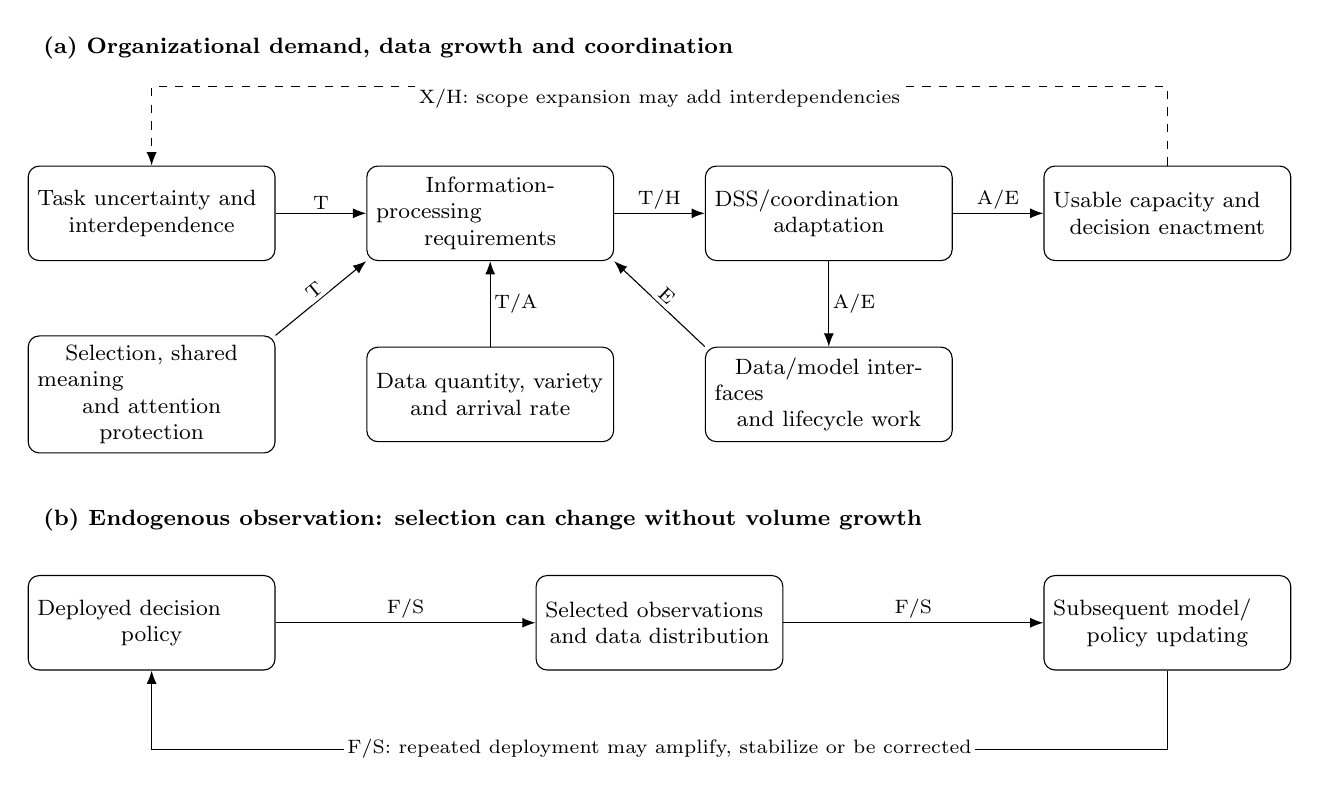
\begin{tikzpicture}[>=Latex, every node/.style={font=\footnotesize}, box/.style={draw,rounded corners,align=center,text width=29mm,minimum height=12mm}, lab/.style={font=\scriptsize,align=center,fill=white,inner sep=1.3pt}]
\node[font=\bfseries\footnotesize,anchor=west] at (-1.5,2.1) {(a) Organizational demand, data growth and coordination};
\node[box] (c) at (0,0) {Task uncertainty and\newline interdependence};
\node[box] (r) at (4.3,0) {Information-processing\newline requirements};
\node[box] (a) at (8.6,0) {DSS/coordination\newline adaptation};
\node[box] (w) at (12.9,0) {Usable capacity and\newline decision enactment};
\node[box] (b) at (0,-2.3) {Selection, shared meaning\newline and attention protection};
\node[box] (v) at (4.3,-2.3) {Data quantity, variety\newline and arrival rate};
\node[box] (g) at (8.6,-2.3) {Data/model interfaces\newline and lifecycle work};
\draw[->] (c) -- node[lab,above] {T} (r);
\draw[->] (r) -- node[lab,above] {T/H} (a);
\draw[->] (a) -- node[lab,above] {A/E} (w);
\draw[->] (a) -- node[lab,right] {A/E} (g);
\draw[->] (g.north west) -- node[lab,sloped,above] {E} (r.south east);
\draw[->] (v) -- node[lab,right] {T/A} (r);
\draw[->] (b.north east) -- node[lab,sloped,above] {T} (r.south west);
\draw[->,dashed] (w.north) -- ++(0,10mm) -| (c.north);
\node[lab] at (6.45,1.45) {X/H: scope expansion may add interdependencies};
\node[font=\bfseries\footnotesize,anchor=west] at (-1.5,-3.9) {(b) Endogenous observation: selection can change without volume growth};
\node[box] (p) at (0,-5.2) {Deployed decision\newline policy};
\node[box] (d) at (6.45,-5.2) {Selected observations\newline and data distribution};
\node[box] (u) at (12.9,-5.2) {Subsequent model/\newline policy updating};
\draw[->] (p) -- node[lab,above] {F/S} (d);
\draw[->] (d) -- node[lab,above] {F/S} (u);
\draw[->] (u.south) -- ++(0,-10mm) -| (p.south);
\node[lab] at (6.45,-6.8) {F/S: repeated deployment may amplify, stabilize or be corrected};
\end{tikzpicture}}
\caption{Conditional mechanism map. T: organizational theory; H: historical synthesis; A: architectural/engineering analysis; E: organizational case evidence; F: formal analysis; S: simulation; X: cross-study conjecture. Labels identify support types, not equal evidence strength. Panel (a) separates volume-related demands from coordination costs; modularity and slack provide additional balancing routes discussed in the text. Panel (b) represents a distinct observation loop, not a necessary increase in organizational work. Connections between panels require context-specific evidence. No loop gain, delay or net complexity change is estimated.}
\label{fig:mechanisms}
\end{figure*}

\section{Cross-Level Illustrations and Critical Comparison}
\subsection{Enterprise Warehousing: Local Acceleration and Deferred Integration}
The warehouse case illustrates the same tension before machine learning. Departmental marts can provide timely analysis while avoiding the delay of enterprise-wide consensus. Their later integration may become difficult if local models diverge \cite{chaudhuri1997}. The short-run advantage is local autonomy and access; the possible long-run cost is reconciling definitions, histories and dependencies. The mechanism is deferred coordination, rather than a direct effect of record count alone.

Shared enterprise architecture can dampen the loop by establishing common dimensions and responsibilities. Yet the source is a technical tutorial, not a longitudinal comparison estimating whether centralized or decentralized warehousing is organizationally superior. Its role is to identify an architecture-dependent mechanism and a rival pathway. A causal test would need the pre-existing reconciliation burden as well as new integration costs; measuring warehouse size or query latency alone would miss the proposed organizational effect.

\subsection{Integrated Care: More Accessible Data, Persistent Situated Judgment}
Greenhalgh \emph{et al.}'s NASSS research combines theory with six health/social-care technology cases, drawing on over 400 hours of observation, 165 interviews and 200 documents \cite{Greenhalgh2017}. Its scope is wider than DSS, so transfer is clearest in the integrated-case-management example rather than every technology discussed. In that case, an organization introduced a warehouse with predictive risk modeling to identify people at high risk of hospital admission and facilitate shared care plans. Actual identification combined model outputs with clinical judgment; plans also circulated outside the warehouse.

This directly illustrates the relationship between interdependent care, shared data and decision support. It also challenges the presumption that technical integration fully integrates work. Professionals still interpret priorities and communicate through situated channels. In the remote biomarker case, repeated measurements and alerts interact with staff engagement, patient understanding, connectivity and support work. The source does not quantify a growth trajectory in data volume or isolate a DSS-caused change in organization-wide complexity. It supports contextual adaptation and limits to technological substitution.

Sutton \emph{et al.}'s clinical DSS review provides a complementary secondary account of alert fatigue, fragmented workflows, changing knowledge bases and interoperability \cite{Sutton2020}. Alert overload is an attention-facing information problem, not the same measurement as archive size. Standardization and integration may help, while excessive low-value notifications can undermine use. The sources together show both benefits and burdens, without supporting a pooled effectiveness estimate or a rule that all monitoring increases complexity.

\subsection{Production ML: New Capacity and Interteam Coupling}
Amershi \emph{et al.}'s Microsoft study uses 14 interviews followed by 551 survey responses to investigate ML engineering practices \cite{amershi2019}. It documents loops among collection, training, evaluation and monitoring, and additional challenges in collaboration and lifecycle support. In particular, changes to diagnostic data collection can require upstream engineering work; coupled model behavior can force separately organized teams to coordinate.

This is actual organizational evidence for a reverse dependency pathway. However, the sample is self-selected and self-reported within one corporation, and it is not limited to applications labeled DSS. Its transfer concerns the production of data-dependent decision components, not a population-wide effect on managerial decisions. Maturing practices can also help teams manage the new work. Sculley's engineering taxonomy explains why such burdens may be easy to overlook, but supplies no independent controlled estimate of their size \cite{sculley2015}.

Across the cases, the consistent observation is redistribution of information work. Warehousing moves reconciliation into shared data infrastructure; integrated care combines formal data with professional coordination; ML introduces data/model lifecycle work across teams. The evidence is weaker for the stronger claim that total organizational complexity necessarily rises. Formal and simulated observation loops add a different result: the system can change the evidence it later consumes, even without an increase in organizational size or record volume. Combining these levels is useful only if those distinctions are retained.

\section{Propositions and Design Implications}
The following propositions are derived from the synthesis, not newly tested empirical findings. Table~\ref{tab:claims} links the central relationships to evidence and limits.

\subsection{P1: Misfit Depends on Interdependence and Meaning}
When task uncertainty or reciprocal interdependence increases beyond what existing plans and coordination arrangements can absorb, information-processing requirements rise; the appropriate response depends on whether the deficit concerns missing evidence, conflicting interpretation, or authority to act \cite{GALBRAITH1974,TUSHMAN1978,DAFT1986}. More records are more likely to help a well-specified missing-fact problem than unresolved equivocality. The proposition predicts that similar data volumes can produce different DSS demands across organizational contexts.

The design implication is to diagnose the constraint before selecting an architecture. Search/aggregation may suit missing evidence; common definitions and discussion may suit conflicting meaning; decision-right clarification may be necessary where no component has authority. Treating all three as a storage or inference problem can produce a technically larger but organizationally less usable system.

\subsection{P2: Coupling Moderates the Cost of Data Expansion}
When expanded data and model use introduces cross-unit dependencies faster than interfaces, ownership and maintenance practices stabilize them, additional analytical capacity can increase coordination work \cite{chaudhuri1997,amershi2019,sculley2015}. This is an additional-work proposition with an undetermined net effect, not a claim that all integration is harmful. Stable semantics and boundaries may remove more reconciliation than they create.

The implication is to assess what new work is created, who performs it, and which existing work disappears. Change-impact analysis should include data consumers, collection regimes and model dependencies, alongside code modules. Query response time and model accuracy alone cannot reveal this balance.

\subsection{P3: More Records Need Not Mean Less Biased Evidence}
When a DSS affects allocation or user behavior, subsequent observations are partly policy-dependent. Additional records may reinforce selection effects or make evaluation on similarly generated data misleading \cite{perdomo2020,chaney2018,ensign2018}. The sign and magnitude depend on sensitivity, external observations and correction mechanisms; the formal/simulation evidence does not establish a universal field effect.

The implication is to record the policy and context of collection, separate observed from underlying activity, and seek appropriately independent or policy-aware evaluation. Monitoring data volume without monitoring the observation process can miss the principal feedback risk. There can also be stable adaptation, so a detected loop should trigger investigation rather than an automatic prediction of instability.

\subsection{P4: Selectivity Can Improve Support While Reducing Exposure}
Where irrelevant detail or low-value, redundant notifications dominate recipient attention, filtering, sampling, understandable models and selective retrieval can increase usable capacity without increasing human information exposure \cite{SIMON1971,little1969,gorry1971,Lewis2020}. The proposition connects older attention/model-design arguments to current access mechanisms; it does not imply that retrieval automatically makes an answer correct or preserves every important exception.

The implication is to distinguish archive growth from interface burden. A larger searchable corpus can coexist with concise presentation; conversely, a modest database can generate an overwhelming notification stream. Evaluation should check missed consequential signals and the costs of selection alongside time saved.

\subsection{P5: Scope Expansion Closes a Reinforcing Loop Only Conditionally}
If improved support enables additional products, partners or delegated decisions that introduce new interdependencies and recording requirements, a reinforcing demand--capacity--scope loop may emerge. The reviewed historical forecasts and bounded coordination evidence make this plausible, but no included study directly tests the complete long-run loop \cite{shim2002,amershi2019}. Expansion is therefore a conjectural closure, not the principal established result.

The implication is to specify the organizational boundary and compare expansion with plausible alternatives. A system may instead stabilize operations, substitute for existing coordination, support downsizing or be abandoned. Successful deployment does not itself demonstrate growth in complexity; failure does not demonstrate absence of the underlying demand.

\begin{table*}[t]
\caption{Evidence-to-mechanism map: support is link-specific, not proof of the full historical loop}
\label{tab:claims}
\centering\footnotesize\setlength{\tabcolsep}{4pt}
\begin{tabular}{p{.23\textwidth}p{.29\textwidth}p{.18\textwidth}p{.22\textwidth}}
\toprule
Relationship & Assessed support and locations & Evidence type & Main boundary / countercondition \\
\midrule
Interdependence/uncertainty increases processing requirements & Galbraith, pp.28--32; Tushman/Nadler, pp.615--617 \cite{GALBRAITH1974,TUSHMAN1978} & Organizational theory & Reduce interdependence or use slack; not a byte-growth law \\
Data growth can strain integration/interpretation & Chaudhuri/Dayal, pp.65--67; Fayyad \emph{et al.}, pp.37--42 \cite{chaudhuri1997,fayyad1996} & Architecture and process synthesis & Selection, semantics and workload matter; no universal causal effect size \\
Data-dependent capability creates lifecycle coordination & Amershi \emph{et al.}, PDF pp.8--9; Sculley \emph{et al.}, Secs.2--4 \cite{amershi2019,sculley2015} & Organizational case plus engineering analysis & Single-organization/self-report limits; added work may replace existing work \\
Decision policies change future observations & Perdomo \emph{et al.}, Secs.2--4; Chaney \emph{et al.}, Sec.5; Ensign \emph{et al.}, Secs.3--5 \cite{perdomo2020,chaney2018,ensign2018} & Formal analysis and simulation & Selection/distribution change is not necessarily volume or complexity growth; stability/correction possible \\
Abstraction and selection can reduce burden & Gorry/Scott Morton, scan p.25; Simon, pp.40--46; Little, scan pp.15--23 \cite{gorry1971,SIMON1971,little1969} & Conceptual/design evidence & Over-filtering can omit relevant exceptions; benefit is decision-specific \\
Capability-enabled scope expansion closes a reinforcing loop & Shim \emph{et al.}, pp.113,122; integration with bounded coordination findings \cite{shim2002,amershi2019} & Historical forecast and review synthesis & Whole-loop conjecture; no included longitudinal test establishes general historical closure \\
\bottomrule
\end{tabular}
\end{table*}

\section{Rival Explanations and Research Agenda}
\subsection{Common Causes and Alternative Trajectories}
Co-occurrence of more complex work, more data and newer DSS is insufficient to infer the proposed feedback. Environmental change, digitization, regulation or changes in organizational scope could produce all three. Resources and managerial priorities could drive both technology investment and restructuring. These alternatives are not estimated in this review; they define what a causal study would need to distinguish.

Reverse causality also requires care. A complex organization may invest in analytics, while analytics may permit coordination at greater scope. Observing the second after the first does not identify the relative contribution. Furthermore, organizational complexity can be relocated: outsourcing a data service may simplify one unit's workflow while increasing interorganizational dependencies. A stable enterprise total can conceal shifts across departments or external partners.

Other trajectories directly challenge a monotonic narrative. Standardization can reduce variety; modularity can reduce reciprocal dependencies; learning can routinize exceptions; budget constraints can prevent collection or investment. Clinical implementation evidence includes workarounds, nonadoption and abandonment, not just successful expansion \cite{Greenhalgh2017}. A review centered only on growing systems would miss these cases and overstate technological inevitability.

\subsection{Operationalizing the Relationships}
Future studies should measure the constructs separately. Data volume could use observations per decision window or archive size, with duplication and collection-policy changes recorded. Data variety could use source/schema diversity; attention exposure could use alerts or items inspected per decision. Organizational interdependence could be assessed through cross-unit handoffs, reciprocal dependencies and escalation paths. Equivocality would require evidence of competing interpretations, not simply prediction variance. These are proposed measurement options, not validated instruments supplied by this review.

Usable capacity should be examined through the time and work needed for a correct coordinated action, including validation and maintenance. Candidate outcomes include decision timeliness, errors relative to specified objectives, reconciliation work, change-impact scope and ability to correct the system. Human and infrastructure costs should be reported separately. No single accuracy or latency number captures all these dimensions.

Longitudinal comparative cases are particularly suitable for tracing when information requirements changed, when a support arrangement changed, and which dependencies were removed or created. Variation in rollout timing may help compare similar organizational units, but identification requires examining prior trends and concurrent changes. Qualitative process tracing can reveal selection and interpretation mechanisms even where a credible numerical causal estimate is unavailable.

For the endogenous-observation loop, studies should track whether data arose independently or through the policy's allocation and presentation decisions. Formal stability results motivate testing sensitivity and correction conditions, not assuming that a simulated result will transfer unchanged. For the scope-expansion conjecture, evidence would need to show that new DSS capability actually enabled activities that then generated additional interdependencies; simple temporal succession is inadequate.

\subsection{Testing Whether Scaling or Redesign Helps}
An evaluation can compare increased resources within the same design with an alternative representation or coordination arrangement at a transparent cost. This need not require matched budgets in every historical case, but resource and workflow changes should be reported. A warehouse redesign may reduce repeated reconciliation without reducing raw records. A selective interface may reduce attention exposure while retaining archive coverage. A decision-right change may resolve a bottleneck that neither extra storage nor a larger model can address.

The key discriminator is what constraint changed and which outcome followed. Cross-sectional comparisons of newer versus older systems confound architecture, organizational maturity, resources and selection. Carefully documented failures and simplifications are as informative as successful expansions because they test the conditions under which the proposed loops do not close.

\section{Limitations}
The review is purposive and access-dependent, with a bounded English-language corpus and targeted search routes. Important candidates remained inaccessible, including several classic DSS papers, business-intelligence reviews and information-overload work; the supplement records those omissions. The initial catalog and exact-title discovery can favor familiar sources. No claim of exhaustive theoretical or historical coverage is made. Reading full-text mechanisms and checking metadata reduces, but does not remove, extraction error; OCR and AI-assisted synthesis introduce additional risks.

The evidence is heterogeneous and uneven across links. Core organizational theories are conceptual; historical sources combine descriptions, examples and forecasts; recent feedback sources are often mathematical or simulated. The strongest organizational examples concern healthcare and production ML, rather than representative samples of all DSS. Generalizing across sector, scale, institutional setting and organizational boundary remains an analytical judgment. The source roles and tables make that judgment inspectable but do not validate it empirically.

The framework does not estimate time delays, net complexity changes, historical adoption rates or comparative effect sizes. It cannot identify the dominant cause of each transition or establish the complete feedback loop. Recent generative/tool-using systems provide mechanism examples with limited long-term organizational evidence here. Finally, identifying close prior reviews does not establish exhaustive novelty. The proposed contribution is the conditional integration and explicit evidence boundary, which remains open to scholarly challenge.

\section{Conclusion}
The evolution of DSS can be understood as repeated adaptation of information-processing arrangements to changing organizational requirements and data conditions. Interdependence and uncertainty create processing demands; growing data can increase integration and interpretation work; technical and organizational responses can expand usable capacity or reduce the demands themselves. Architectures matter because they redistribute work across models, stores, interfaces, people and organizational boundaries.

Feedback adds two supported qualifications to a simple progress narrative. Decision policies can alter future observations, and data-dependent systems can introduce new coordination and lifecycle obligations. Neither result means that more records inevitably create greater organizational complexity. Sampling, abstraction, shared meaning, modularity and corrective observation can balance the relationship. The stronger claim that DSS-enabled expansion closes a self-reinforcing historical loop remains conditional and incompletely tested.

A defensible design strategy therefore begins by identifying whether the constraint concerns missing evidence, interpretation, attention, throughput or coordinated action. Scaling, redesign and simplification are alternative responses whose value depends on those conditions. This review offers an evidence-linked framework for investigating that choice, rather than a universal technological sequence or a measured law of organizational growth.

\section*{AI Assistance and Authorship}
Literature discovery, text extraction, synthesis checking, manuscript drafting and document preparation were assisted by AI tools. The manuscript remains unattributed as requested; it reports no new experiments or human-participant data collection. Responsibility for submission, authorship, source verification and the selected venue's disclosure requirements rests with the eventual human authors.

\begin{thebibliography}{24}
\bibitem{GALBRAITH1974} J. R. Galbraith, ``Organization Design: An Information Processing View,'' \emph{Interfaces}, vol. 4, no. 3, pp. 28--36, 1974, doi: 10.1287/inte.4.3.28. [Online]. Available: \url{https://doi.org/10.1287/inte.4.3.28}
\bibitem{TUSHMAN1978} M. L. Tushman and D. A. Nadler, ``Information Processing as an Integrating Concept in Organizational Design,'' \emph{Academy of Management Review}, vol. 3, no. 3, pp. 613--624, 1978, doi: 10.5465/amr.1978.4305791. [Online]. Available: \url{https://doi.org/10.5465/amr.1978.4305791}
\bibitem{shim2002} J. P. Shim, M. Warkentin, J. F. Courtney, D. J. Power, R. Sharda and C. Carlsson, ``Past, Present, and Future of Decision Support Technology,'' \emph{Decision Support Systems}, vol. 33, no. 2, pp. 111--126, 2002, doi: 10.1016/S0167-9236(01)00139-7. [Online]. Available: \url{https://scholarworks.uni.edu/facpub/3462/}
\bibitem{power2004} D. J. Power, ``Specifying an Expanded Framework for Classifying and Describing Decision Support Systems,'' \emph{Communications of the Association for Information Systems}, vol. 13, pp. 158--166, 2004, doi: 10.17705/1CAIS.01313. [Online]. Available: \url{https://aisel.aisnet.org/cais/vol13/iss1/13/}
\bibitem{perdomo2020} J. C. Perdomo, T. Zrnic, C. Mendler-D\"{u}nner and M. Hardt, ``Performative Prediction,'' in \emph{Proceedings of the 37th International Conference on Machine Learning}, Proceedings of Machine Learning Research, vol. 119, pp. 7599--7609, 2020. [Online]. Available: \url{https://proceedings.mlr.press/v119/perdomo20a.html}
\bibitem{amershi2019} S. Amershi \emph{et al.}, ``Software Engineering for Machine Learning: A Case Study,'' in \emph{2019 IEEE/ACM 41st International Conference on Software Engineering: Software Engineering in Practice (ICSE-SEIP)}, pp. 291--300, 2019, doi: 10.1109/ICSE-SEIP.2019.00042. [Online]. Available: \url{https://doi.org/10.1109/ICSE-SEIP.2019.00042}
\bibitem{little1969} J. D. C. Little, ``Models and Managers: The Concept of a Decision Calculus,'' MIT Sloan School of Management Working Paper, Rep. 403-69, June 1969. [Online]. Available: \url{https://archive.org/details/modelsmanagersco00litt}
\bibitem{gorry1971} G. A. Gorry and M. S. Scott Morton, ``A Framework for Management Information Systems,'' MIT Sloan School of Management Working Paper, Rep. 510-71, February 1971. [Online]. Available: \url{https://archive.org/details/frameworkformana00gorr}
\bibitem{arnott2008} D. Arnott and G. Pervan, ``Eight Key Issues for the Decision Support Systems Discipline,'' \emph{Decision Support Systems}, vol. 44, pp. 657--672, 2008, doi: 10.1016/j.dss.2007.09.003. [Online]. Available: \url{https://www.sciencedirect.com/science/article/pii/S0167923607001698}
\bibitem{Budianto2026} F. A. Budianto, M. Lubis, I. Y. Mukti and S. Budianto, ``The Evolution of Decision Support Systems (DSS) to Strategic AI: A Systematic Review of Architectural Shifts and Business Value,'' \emph{RIGGS: Journal of Artificial Intelligence and Digital Business}, vol. 5, no. 1, pp. 8905--8916, 2026, doi: 10.31004/riggs.v5i1.6990. [Online]. Available: \url{https://journal.ilmudata.co.id/index.php/RIGGS/article/download/6990/5330}
\bibitem{Eze2026} E. J. Eze, F. M. Bello and O. T. Akinyemi, ``Decision Support Systems: Evolution, Architectures, Applications, and Future Directions,'' \emph{Data Intelligence and Informatics Practice}, vol. 1, no. 1, pp. 19--31, 2026, doi: 10.53623/diip.v1i1.1264. [Online]. Available: \url{https://tecnoscientifica.com/journal/diip/article/download/1264/626}
\bibitem{DAFT1986} R. L. Daft and R. H. Lengel, ``Organizational Information Requirements, Media Richness and Structural Design,'' \emph{Management Science}, vol. 32, no. 5, pp. 554--571, 1986, doi: 10.1287/mnsc.32.5.554. [Online]. Available: \url{https://doi.org/10.1287/mnsc.32.5.554}
\bibitem{SIMON1971} H. A. Simon, ``Designing Organizations for an Information-Rich World,'' in \emph{Computers, Communications, and the Public Interest}, M. Greenberger, Ed. Baltimore, MD, USA: The Johns Hopkins Press, 1971, pp. 37--72. [Online]. Available: \url{https://digitalcollections.library.cmu.edu/awweb/awarchive?type=file&item=33748}
\bibitem{feigenbaum1977} E. A. Feigenbaum, ``The Art of Artificial Intelligence: Themes and Case Studies of Knowledge Engineering,'' in \emph{Proceedings of the Fifth International Joint Conference on Artificial Intelligence}, pp. 1014--1029, 1977. [Online]. Available: \url{https://www.ijcai.org/proceedings/1977/}
\bibitem{Sutton2020} R. T. Sutton, D. Pincock, D. C. Baumgart, D. C. Sadowski, R. N. Fedorak and K. I. Kroeker, ``An overview of clinical decision support systems: benefits, risks, and strategies for success,'' \emph{npj Digital Medicine}, vol. 3, Art. no. 17, 2020, doi: 10.1038/s41746-020-0221-y. [Online]. Available: \url{https://www.nature.com/articles/s41746-020-0221-y}
\bibitem{chaudhuri1997} S. Chaudhuri and U. Dayal, ``An Overview of Data Warehousing and OLAP Technology,'' \emph{ACM SIGMOD Record}, vol. 26, no. 1, pp. 65--74, 1997, doi: 10.1145/248603.248616. [Online]. Available: \url{https://sigmodrecord.org/1997/03/15/an-overview-of-data-warehousing-and-olap-technology/}
\bibitem{fayyad1996} U. Fayyad, G. Piatetsky-Shapiro and P. Smyth, ``From Data Mining to Knowledge Discovery in Databases,'' \emph{AI Magazine}, vol. 17, no. 3, pp. 37--54, 1996, doi: 10.1609/aimag.v17i3.1230. [Online]. Available: \url{https://ojs.aaai.org/aimagazine/index.php/aimagazine/article/view/1230}
\bibitem{Dean2004} J. Dean and S. Ghemawat, ``MapReduce: Simplified Data Processing on Large Clusters,'' in \emph{Proceedings of the 6th Symposium on Operating Systems Design and Implementation}, 2004. [Online]. Available: \url{https://research.google/pubs/mapreduce-simplified-data-processing-on-large-clusters/}
\bibitem{sculley2015} D. Sculley \emph{et al.}, ``Hidden Technical Debt in Machine Learning Systems,'' \emph{Advances in Neural Information Processing Systems}, vol. 28, 2015. [Online]. Available: \url{https://papers.nips.cc/paper_files/paper/2015/hash/86df7dcfd896fcaf2674f757a2463eba-Abstract.html}
\bibitem{Lewis2020} P. Lewis \emph{et al.}, ``Retrieval-Augmented Generation for Knowledge-Intensive NLP Tasks,'' \emph{arXiv:2005.11401}, 2020. [Online]. Available: \url{https://arxiv.org/abs/2005.11401}
\bibitem{Yao2023} S. Yao \emph{et al.}, ``ReAct: Synergizing Reasoning and Acting in Language Models,'' in \emph{Proceedings of the International Conference on Learning Representations}, 2023. [Online]. Available: \url{https://arxiv.org/abs/2210.03629}
\bibitem{chaney2018} A. J. B. Chaney, B. M. Stewart and B. E. Engelhardt, ``How Algorithmic Confounding in Recommendation Systems Increases Homogeneity and Decreases Utility,'' in \emph{Proceedings of the 12th ACM Conference on Recommender Systems}, pp. 224--232, 2018, doi: 10.1145/3240323.3240370. [Online]. Available: \url{https://doi.org/10.1145/3240323.3240370}
\bibitem{ensign2018} D. Ensign, S. A. Friedler, S. Neville, C. Scheidegger and S. Venkatasubramanian, ``Runaway Feedback Loops in Predictive Policing,'' in \emph{Proceedings of the 1st Conference on Fairness, Accountability and Transparency}, Proceedings of Machine Learning Research, vol. 81, pp. 160--171, 2018. [Online]. Available: \url{https://proceedings.mlr.press/v81/ensign18a.html}
\bibitem{Greenhalgh2017} T. Greenhalgh \emph{et al.}, ``Beyond Adoption: A New Framework for Theorizing and Evaluating Nonadoption, Abandonment, and Challenges to the Scale-Up, Spread, and Sustainability of Health and Care Technologies,'' \emph{Journal of Medical Internet Research}, vol. 19, no. 11, Art. no. e367, 2017, doi: 10.2196/jmir.8775. [Online]. Available: \url{https://www.jmir.org/2017/11/e367/}
\end{thebibliography}
\end{document}
